\section{Lagrange Polynomial Interpolation}

This general theory describes construction of polynomial interpolatory basis for simplex geometries. \textbf{[wiki-lagrange]}. The general idea is to describe the real geometry of the curved entity in global coordinates as a mapping $\vec{p}(\vec{r})$ of its local geometry, which is a basic linear geometry called a reference element. \\

\noindent
Using the Dune-convention, a reference simplices are defined by
\begin{itemize}
	\item $\Delta_0 : \{ \}$
	\item $\Delta_1 : \{ 0\}, \{ 1\}$
	\item $\Delta_2 : \{ 0, 0 \}, \{ 1, 0 \}, \{ 0, 1 \}$
	\item $\Delta_3 : \{ 0, 0, 0 \}, \{ 1, 0, 0 \}, \{ 0, 1, 0 \}, \{ 0, 0, 1 \}$
\end{itemize}

\noindent
Local simplex geometries can be parameterized using the local coordinate vector $\vec{r}$:
\begin{itemize}
	\item edge:			$\vec{r}=(u)$,		such that $u \in [0,1]$
	\item triangle: 	$\vec{r}=(u,v)$,	such that $u \in [0,1]$ and $v \in [0, 1-u]$
	\item tetrahedron:	$\vec{r}=(u,v,w)$,	such that $u \in [0,1]$, $v \in [0, 1-u]$ and $w \in [0, 1-u-v]$ 
\end{itemize}

\subsection{Interpolatory Vertices}

\noindent
In order to define the curvilinear geometry, a set of real geometry points $\vec{p}_i(\vec{r}_i)$ is provided, over which the real geometry is interpolated. By convention, the real geometry is sampled over a rectangular grid over the reference simplex, namely
\[\vec{r}_{i,j,k} = \frac{(i,j,k)}{Ord}, \;\;\; i=[0..Ord], \;\;\; j=[0..Ord-i], \;\;\; k=[0..Ord-i-j]\]
where $Ord$ is the interpolation order of the surface. Thus, points from this uniform grid in local coordinates are mapped to arbitrary points in global coordinates. It is the job of the meshing software (in our case GMSH) to ensure that the global geometry is non-singular / non-self-intersecting. The uniform convention is taken by GMSH mostly because polynomial orders remain rather low. If higher orders would be required, a non-uniform (e.g. Chebyshev) sampling grid would have to be used in order to minimize the Runge phenomenon. \\

\noindent
It is easy to verify that the above discretization generates the following number of interpolatory points as a function of interpolatory order (starting with 1, mentioning first 5 orders)
\begin{itemize}
	\item edge:			$N_{Ord} = \{ 2,3,4,5,6 \}  $
	\item face:			$N_{Ord} = \{ 3,6,10,15,21 \}  $
	\item tetrahedron:	$N_{Ord} = \{ 4,10,20,35,56 \}  $
\end{itemize}

\subsection{Interpolatory Polynomials}
\label{section-interppoly}

\noindent
It is easy to verify, that the number of interpolatory points above exactly matches the total number of monomials necessary to construct a complete polynomial of order $Ord$ or less. Define the functions $z^{(1,i)}(u)$, $z^{(2,i)}(u,v)$ and $z^{(3,i)}(u,v,w)$ as the set of all monomials of corresponding order, where the first parameter is dimension of the entity, and the 2nd is the polynomial order:
\begin{itemize}
	\item edge: \\
		$z^{(1,1)}(u) = \{1, u\}$, \\
		$z^{(1,2)}(u) = \{1, u, u^2\}$, \\
		$z^{(1,3)}(u) = \{1, u, u^2, u^3\}$, \\
		$z^{(1,4)}(u) = \{1, u, u^2, u^3, u^4\}$, \\
		$z^{(1,5)}(u) = \{1, u, u^2, u^3, u^4, u^5\}$, \\
		etc
	\item face:	\\
		$z^{(2,1)}(u,v)	= \{1, u, v\}$, \\
		$z^{(2,2)}(u,v) = \{1, u, v, u^2, uv, v^2\}$, \\
		etc
	\item tetrahedron: \\
		$z^{(2,1)}(u,v,w) = \{1, u, v, w\}$, \\ 
		$z^{(2,2)}(u,v,w) = \{1, u, v, w, u^2, uv, v^2, wu, wv, w^2\}$, \\
		etc
\end{itemize}

\noindent
This means that using such grid sampling allows using complete polynomials of a given order for interpolation. If one interpolates over other entities, for example, rectangles, one has to either use an incomplete basis of certain order in order to keep using the rectangular sampling grid convention, or change the sampling convention to have exact number of interpolatory points for a certain order. \textbf{[Volakis2010]} choose the first approach, thus interpolating a 9 node 2nd order rectangle with 4th order incomplete polynomial which has a convenient separable tensor product form. \\

\noindent
\textbf{The main idea of Lagrange Polynomials} is to generate a polynomial vector function $\vec{p}(\vec{r})$, which would correspond to a correct global coordinate $\vec{p}_i = \vec{p}(\vec{r}_i)$ for each local coordinate $\vec{r}_i$. It can be easily seen that such function is unique and must take the form
\begin{equation}
	\vec{p}(\vec{r}) = \sum_j L_j(\vec{r})\vec{p}_j 
\end{equation}
\noindent
where the Lagrange Polynomials $L_j$ are defined by their interpolatory property
\begin{equation}
	\label{equation-lagrangepol-interpolatory-property}
	L_j(\vec{r}_i) = \delta_{ij}
\end{equation}
\noindent
for all interpolatory points $\vec{r}_i$. It is easy to see that the amount of free parameters of each Lagrange Polynomial must be equal to the number of interpolatory points, such that each of them can uniquely interpolate a set of $N_{Ord}$ points ($N_{Ord} - 1$ zeroes and 1 one). As we have discussed above, this is indeed the case, as the number of free parameters of a Lagrange polynomial is equal to the number of monomials \\

\noindent
Next, one slightly tricky part, and then we are done. We would like to prove that the following equation holds:
\begin{equation}
	\label{equation-lagrangepol-basis-link}
	z_i(\vec{r}) = \sum_j L_j(\vec{r}) z_i (\vec{r}_j) 
\end{equation}
\noindent
where $z_i$ is a vector of monomials defined above. This equation should hold for all $z^{(\dim, Ord)}$, where $\dim = \{1,2,3\}$. For $\dim < 3$ where $z$ is defined for less than 3 parameters, simply ignore the extra parameters in $\vec{r}$. \\

\noindent
The proof is quite simple. Both LHS and RHS are polynomials of order at most $Ord$, which means that they have at most $N_{Ord}$ free parameters, and therefore, if we can show that the equation holds for $N_{Ord}$ different parameter sets, then it holds for all others as well. And indeed, \eqref{equation-lagrangepol-basis-link} holds for all $\vec{r} = \vec{r}_k$ because of \eqref{equation-lagrangepol-interpolatory-property}. \\

\noindent
Finally, we can write \eqref{equation-lagrangepol-basis-link} as a vector equation
\begin{equation}
	\vec{z} (\vec{r}) = V \vec{L} (\vec{r})
\end{equation}
\noindent
where $V_{ij} = z_i (\vec{r}_j)$, and find the Lagrange polynomials by inverting $V$, namely
\begin{equation}
	\vec{L} (\vec{r}) = V^{-1} \vec{z} (\vec{r})
\end{equation}
\noindent
Thus each Lagrange Polynomial is a linear combination of standard polynomials. They are polynomials of order (at most) $Ord$. Depending on whether we are dealing with edges, faces or tetrahedrons, $L_j$ will be a function of 1, 2 or 3 parameters.

\subsection{Discussion}

\noindent
Important question is the interpretation of the interpolated manifold
\begin{itemize}
	\item edge: a bounded curve which connects a certain set of points
	\item triangle: a bounded surface which connects a certain set of points
	\item tetrahedron: a bounded volume which connects a certain set of points
\end{itemize}

\noindent
It is important to understand, especially for the tetrahedral case, that the parameterized bounded manifold is not exhaustively defined by the shape of its boundary. In tetrahedral case, interpolation over points associated with the element itself does not only mean that the interpolatory point is located inside of the tetrahedron. What it means that the geometry within the tetrahedron is also curved, such that all points within the parametric reference tetrahedron are uniquely mapped to the points in the real tetrahedron.


\subsection{Implementation for Simplices}
\label{subsection-simplexgrid}

\noindent
In this section we discuss how to efficiently enumerate the simplex interpolatory points, and to construct the reference simplex grid. \\

\noindent
Let us place a set of points $\vec{\eta} \in Z^{\dim}$ over simplex $\Delta^{\dim}_{\mathrm{len}}$. This can be done trivially
by using 3 for loops and pushing vectors into a vector
\begin{itemize}
	\item $\Delta^{1}_n = \{(i)\}$, for $i = [1$ to $n]$
	\item $\Delta^{2}_n = \{(j,i)\}$, for $i = [1$ to $n]$, $j = [1$ to $n - i]$
	\item $\Delta^{3}_n = \{(k,j,i)\}$, for $i = [1$ to $n]$, $j = [1$ to $n - i]$, $k = [1$ to $n - i - j]$
\end{itemize}

\noindent
Then, each point $(\Delta^{d}_n)_i$ corresponds exactly to the power of $u,v,w$ in the expansion of $(1 + u + v + w)^n$, namely
\[ (1 + u)^n = \sum_{i=0}^n C^{(\Delta^{1}_n)_i}_n u^{(\Delta^{1}_n)_{i,1}} \]
\[ (1 + u + v)^n = \sum_{i=0}^n C^{(\Delta^{1}_n)_i}_n u^{(\Delta^{1}_n)_{i,1}} v^{(\Delta^{1}_n)_{i,2}} \]
\[ (1 + u + v + w)^n = \sum_{i=0}^n C^{(\Delta^{1}_n)_i}_n u^{(\Delta^{1}_n)_{i,1}} v^{(\Delta^{1}_n)_{i,2}} w^{(\Delta^{1}_n)_{i,3}} \]

\noindent
where $C^{i}_n, C^{i,j}_n$ and $C^{i,j,k}_n$ are the binomial, trinomial and quatranomial coefficients. The powers of the parameters given in this way are exactly the complete monomial basis for a polynomial of order up to and including $d$. \\

\noindent
Also, it is convenient to note that $(\Delta^{d}_n)_i / n$ is exactly the parametric coordinates of the interpolation points on a regular grid over simplex. 

\begin{figure}[hp]
    \centering
    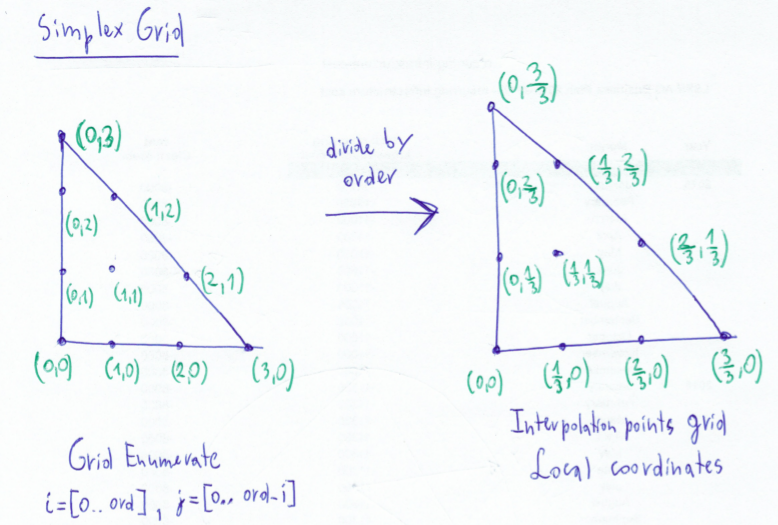
\includegraphics[scale=0.5]{doc-pics/pic-simplex-grid.png}
    %\caption{Awesome Image}
    %\label{fig:awesome_image}
\end{figure}

\noindent
After the monomials and the parametric interpolation points have been constructed, it remains to construct the interpolation matrix by evaluating the monomials at the interpolation points, then to invert the matrix, and multiply the monomial vector by it obtaining lagrange polynomials. This has been implemented both explicitly, by calculating all the lagrange interpolatory polynomials for simplices and writing them as functions, and implicitly, by introducing a polynomial class, which has all the above functionality, and thus generates a set of interpolatory polynomials which can be evaluated and integrated analytically by the code.